\chapter{7 TeV and 8 TeV Differential Cross Section Measurement: Systematic Uncertainties and Results}
\label{c:Differential_Cross_Section:systematics_and_results}

\section{Results}
\label{s:results}

\section{Systematic uncertainties}
\label{s:systematic_uncertainties}
		- How we deal with systematics

\subsubsection{Rate Changing Uncertainties}
\label{sss:rate_changing_uncertainties}

\subsubsection{Shape Changing Uncertainties}
\label{sss:shape_changing_uncertainties}
		
Tau energy: The met energy systematics are electron energy up/down, muon energy up/down and tau energy
up/down. These systematics (and JES) are applied to both monte carlo and data. We found that the tau energy is
susprisingly high, considerably higher than the electron and muon energy systematics. We may select taus in
our signal region unintentionally although we don't select on taus. The signature of ttbar events with taus
can mimic the signature of electron + jets or muon + jets ttbar events. The image shows how taus decay. The W
from a top could decay to a tau, which would then decay either to a tau neutrino and a virtual W which then
decays to two jets which would be very close together (and therefore reconstructed as a single jet). Or, the
virtual W could decay to a lepton (electron or muon) and an associated neutrino). These signatures could fake
our signal, and therefore end up in our ttbar signal. In our unfolding, we remove fakes. However, we use the
shape of the fakes in the central to subtract from the signal distribution in the tau energy up/down
variations. The effect is not so pronounced in the electron up/down and muon up/down variations because there
are not many electrons or muons in the fakes. Luke found that \~14\% of the TTJet events we select on are NOT
from the decay we are looking for. This was by dividing the number of events in the fake ST distribution in
the unfolding histogram file by the number of events in the measured distribution (i.e. signal) in the same
file. The electron channel was actually ~13.5\% and the muon channel was actually ~13.9\%. The shape
comparison between the fakes and the signal shows that there are more fakes in the higher MET bins, which is
why the error in those bins is larger. These are likely to come from semi-leptonic tau events (where the tau
decays to a lepton and a neutrino); tau tau, e tau or mu tau where the tau decays hadronically; or ee, emu or
mumu events where one of the leptons is lost (probably low fraction as well). So most of our fakes will
include at least one tau. Since semi-leptonic tau would need to decay leptonically, these taus are not
identified and, I assume, not included in the MET uncertainty.

Looking at the shape difference between the central and tau up/down MET distributions, there is a significant
different (though not by much). Since this affects data, the difference goes through the fit, and the
unfolding, and is what we see in the final result. The difference in normalisation in the most affected bin is
\~6\%, suggesting that we have more than 6\% tau contamination overall (not sure if that is a correct
assumption). The normalisation across the bins does not change, of course, i.e. the sum of events in the bins
of, in this case MET, remain the same in the central measurement and in the tau energy up/down variations.
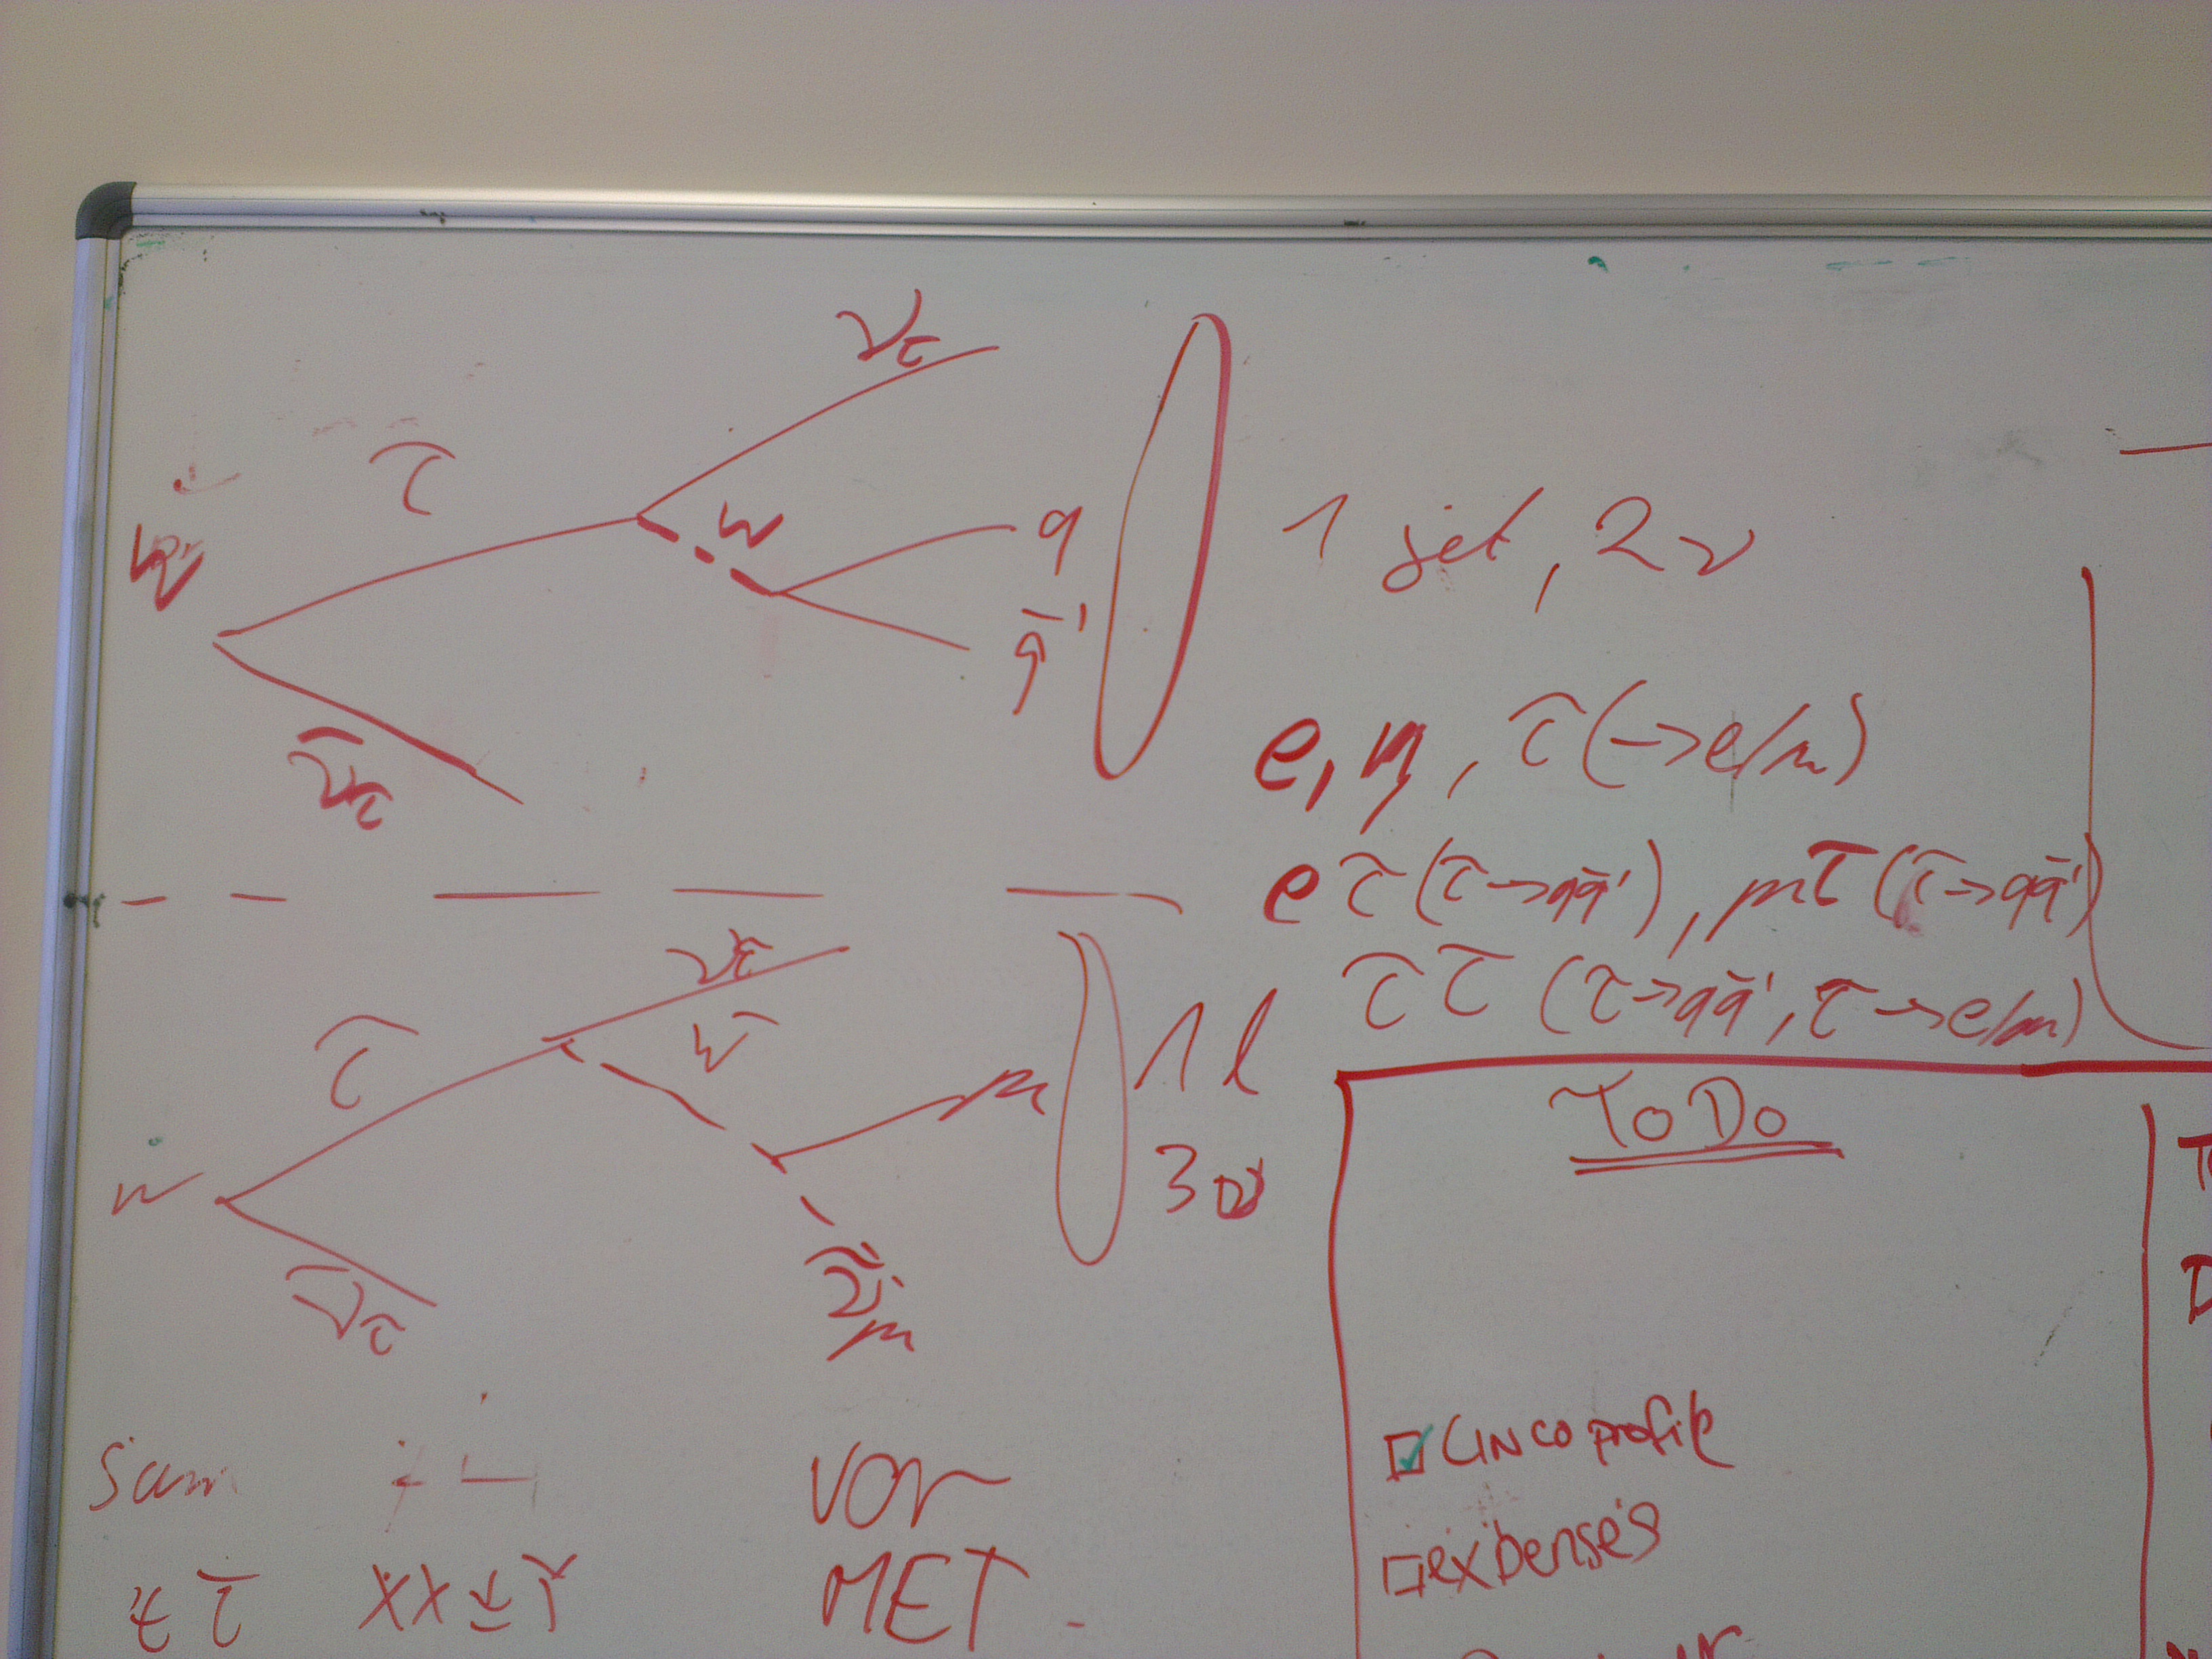
\includegraphics[width=\textwidth]{Chapters/04_Analysis/04b_XSections/Images/IMG_20150219_160840.jpg}

			- theoretical systematics
			- tau systematic

Systematic tables			
	- Results Plots
	- Typical systematics (needed?)
	
	
To put in Appendix:
Results tables